%!TEX root = main.tex
\usepackage{tikz}
\usetikzlibrary{backgrounds,positioning,fit}

% overview of the architecture
\newcommand{\tikzarchitecture}{
  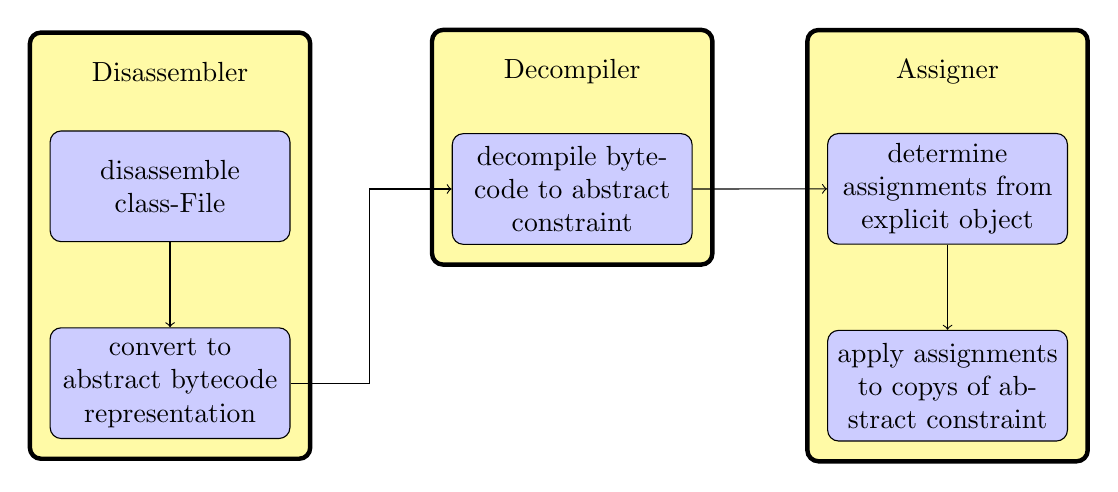
\begin{tikzpicture}[node distance=2.5cm]
    \tikzstyle{block} = [rectangle, draw, fill=blue!20, text width=8em,
        text centered, rounded corners, minimum height=4em]
    \tikzstyle{line} = [draw, ->]
    \tikzstyle{container} = [rectangle, draw, ultra thick, rounded corners,
        inner sep=.25cm, fill=yellow!35]

    % Disassembler
    \node[] (disname) {Disassembler};
    \node[block, below=.5cm of disname] (disassemble) {disassemble class-File};
    \node[block, below of=disassemble] (convert) {convert to abstract bytecode
        representation};
    \draw[line] (disassemble) -- (convert);
    \begin{scope}[on background layer]
      \node[container,fit=(disname) (disassemble) (convert)] (disassembler) {};
    \end{scope}
    % Decompiler
    \node[right=3cm of disname] (decname) {Decompiler};
    \node[block, below=.5cm of decname] (decompile) {decompile bytecode to
        abstract constraint};
    \begin{scope}[on background layer]
      \node[container,fit=(decname) (decompile)] (disassembler) {};
    \end{scope}
    % Assigner
    \node[right=3cm of decname] (assname) {Assigner};
    \node[block, below=.5cm of assname] (assign) {determine assignments from
        explicit object};
    \node[block, below of=assign] (apply) {apply assignments to copys of
        abstract constraint};
    \draw[line] (assign) -- (apply);
    \begin{scope}[on background layer]
      \node[container,fit=(assname) (assign) (apply)] (assigner) {};
    \end{scope}

    \draw[line] (convert.east) -- ++(1,0) |-  (decompile.west);
    \draw[line] (decompile.east) -- (assign.west);
  \end{tikzpicture}
}

\newcommand{\tikzjvm}{
  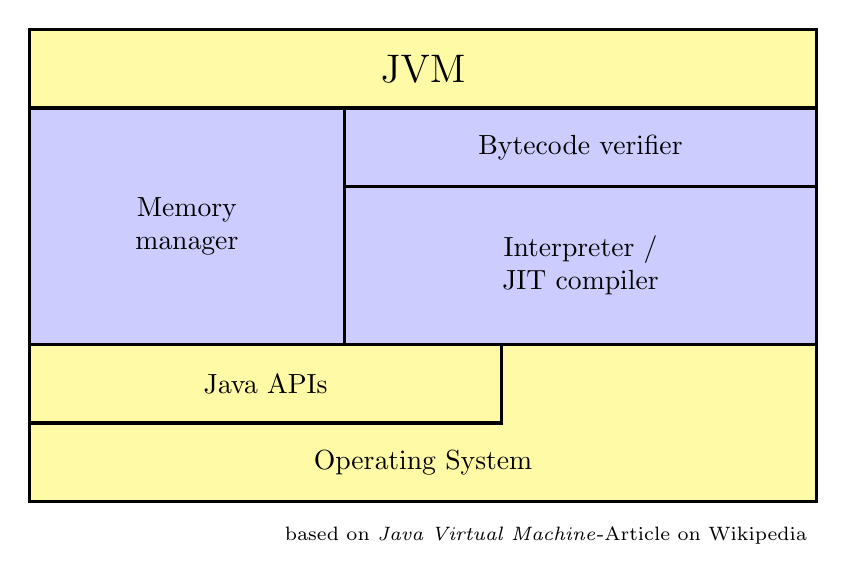
\begin{tikzpicture}
    \draw[very thick,fill=yellow!35] (0,0) rectangle (10,6);

    \draw[very thick] (0,2) rectangle (10,5);
    \draw[very thick] (0,5) rectangle (10,6) node[midway,align=center]
      {\Large JVM};
    \draw[very thick,fill=blue!20] (0,2) rectangle (4,5) node[midway,
      align=center] {Memory\\manager};
    \draw[very thick] (4,2) rectangle (10,5);
    \draw[very thick,fill=blue!20] (4,4) rectangle (10,5) node[midway,
      align=center] {Bytecode verifier};
    \draw[very thick,fill=blue!20] (4,2) rectangle (10,4) node[midway,
      align=center] {Interpreter / \\JIT compiler};
    \draw[very thick] (0,1) rectangle (6,2) node[midway,align=center] {Java
      APIs};
    \draw[very thick] (0,0) rectangle (10,2);
    \draw[draw=none] (0,0) rectangle (10,1) node[midway,align=center]
      {Operating System};

    \draw[draw=none] (0,0) rectangle (10,-.2) node[anchor=north east]
      {\scriptsize based on \emph{Java Virtual Machine}-Article on Wikipedia};
  \end{tikzpicture}
}

%%% Local Variables:
%%% mode: latex
%%% TeX-master: "main"
%%% End:
